% -*- root: ../gvoysey-thesis.tex -*-
\chapter{The Corti Modeling Framework}
\label{chapter:the_corti_modeling_framework}
\thispagestyle{myheadings}

% set this to the location of the figures for this chapter. it may
% also want to be ../Figures/2_Body/ or something. make sure that
% it has a trailing directory separator (i.e., '/')!
\graphicspath{{4_Methods/Figures/}}

\section{Chapter Summary} % (fold)
\label{sec:methodsummary}
This chapter gives a detailed description of Corti, the modeling environment created for this thesis.  \hyperref[sec:overview_of_modeling_framework]{First}, the configuration of the overall system is detailed.  \hyperref[sec:peripheral_models]{Second}, the configuration and use of two models of the auditory periphery are detailed.  \hyperref[sec:auditory_nerve_response_models]{Third}, the creation of compound action potentials and population responses of the auditory nerve are given.  A method for the simulation of cochlear synaptopathy is also detailed, along with a new incorporation of a nonlinear distribution of auditory nerve fiber types as a function of center frequency.  \hyperref[sec:brainstem_models]{Fourth}, the use of these auditory nerve responses in simulation of the auditory brainstem and midbrain with two models are given, culminating in the creation of modeled Auditory Brainstem Responses.  \hyperref[sec:automated_parameter_exploration]{Finally}, the utility of the system for large-scale simulation is shown. 


\section{Overview of Modeling Framework} % (fold)
\label{sec:overview_of_modeling_framework}
The modeling framework created for this thesis has been named Corti \citep{Voysey2016Corti}. It is architecturally inspired by the EarLab project developed at Boston University as well as the Cochlea \citep{Rudnicki2014Cochlea} modeling environment developed at the Technical University of Munich, from which it incorporates a peripheral model.

Corti is a command-line tool written in Python. As detailed in \autoref{fig:corti-overview}, it is designed to produce estimates of the ABR, auditory nerve fiber, CAP, brainstem and midbrain responses to an arbitrary stimulus.  A set of configuration parameters, specified by the user, determine which models are used and how they are interconnected, as well as the spatiotemporal properties of the stimulus.

\subsection{Software Design} % (fold)
\label{sub:software_design}
Corti has been designed to be an easy to use and flexible command-line tool that should be immediately usable to anyone interested in auditory modeling and who is familiar with basic auditory physiology and engineering.  It has a fully documented user interface, requires no special system configuration to use, and runs on Linux, Windows, and OSX.

Corti is publicly available and open source. It is licensed under the GNU GPLv3, and as such is free to distribute, use, and be contributed to by anyone.  The file format used to store large simulation output is the Hierarchal Data Format (HDF5), which is a database-in-a-file that can be analyzed and accessed by any operating system and any modern programming language---while Corti is written in Python, analysis of its output may be done in \textsc{matlab}, R, SPSS or any other modern data analysis tool.

Corti was designed so that its output can be easily audited and examined to know not only which biophysical parameters were used, but also know comprehensive metadata about the simulation itself.  For example, model output contains which version of each model was used, the date and time of the computation, a copy of the stimulus used to stimulate the models, and a comprehensive record of other relevant parameters. 

Additionally, the development history of Corti is publicly accessible on the collaborative software repository website GitHub (\url{https://github.com/gvoysey/corti}).  Every change made, and every version released, is available so direct comparisons between output can be made, and software bugs fixed in a central location.  A permanent archive of the version of Corti described in this thesis has been assigned a Document Object Identifier (DOI), and is available via Zenodo (\url{https://zenodo.org/record/57111}), which is an EU and CERN funded research data repository.  At the time of this writing, Corti has been used to run simulations by research groups at Boston~University, the Massachusetts~General~Hospital, the Carl~von~Ossietzky~University~of~Oldenburg, and the Technical~University~of~Denmark.  

\subsection{Configuration Options Define a Parameter Space}
As detailed in \autoref{chapter:literaturereview}, the constituent models of this framework each require many choices of user-selected parameters, ranging from sampling frequency to the time constants and relative strength and latency of inhibitory and excitatory contributions of brainstem areas. Several other parameters are introduced in the framework itself, as well as the choice of which model to use for each stage. Because these parameter choices directly modulate the simulation output, it quickly becomes natural to treat these different options as a high-dimensional parameter space.  

Any single run of the framework, using one collection of user-specified options, defines a particular trajectory though this space.

\begin{figure}[htbp]
	\centering
	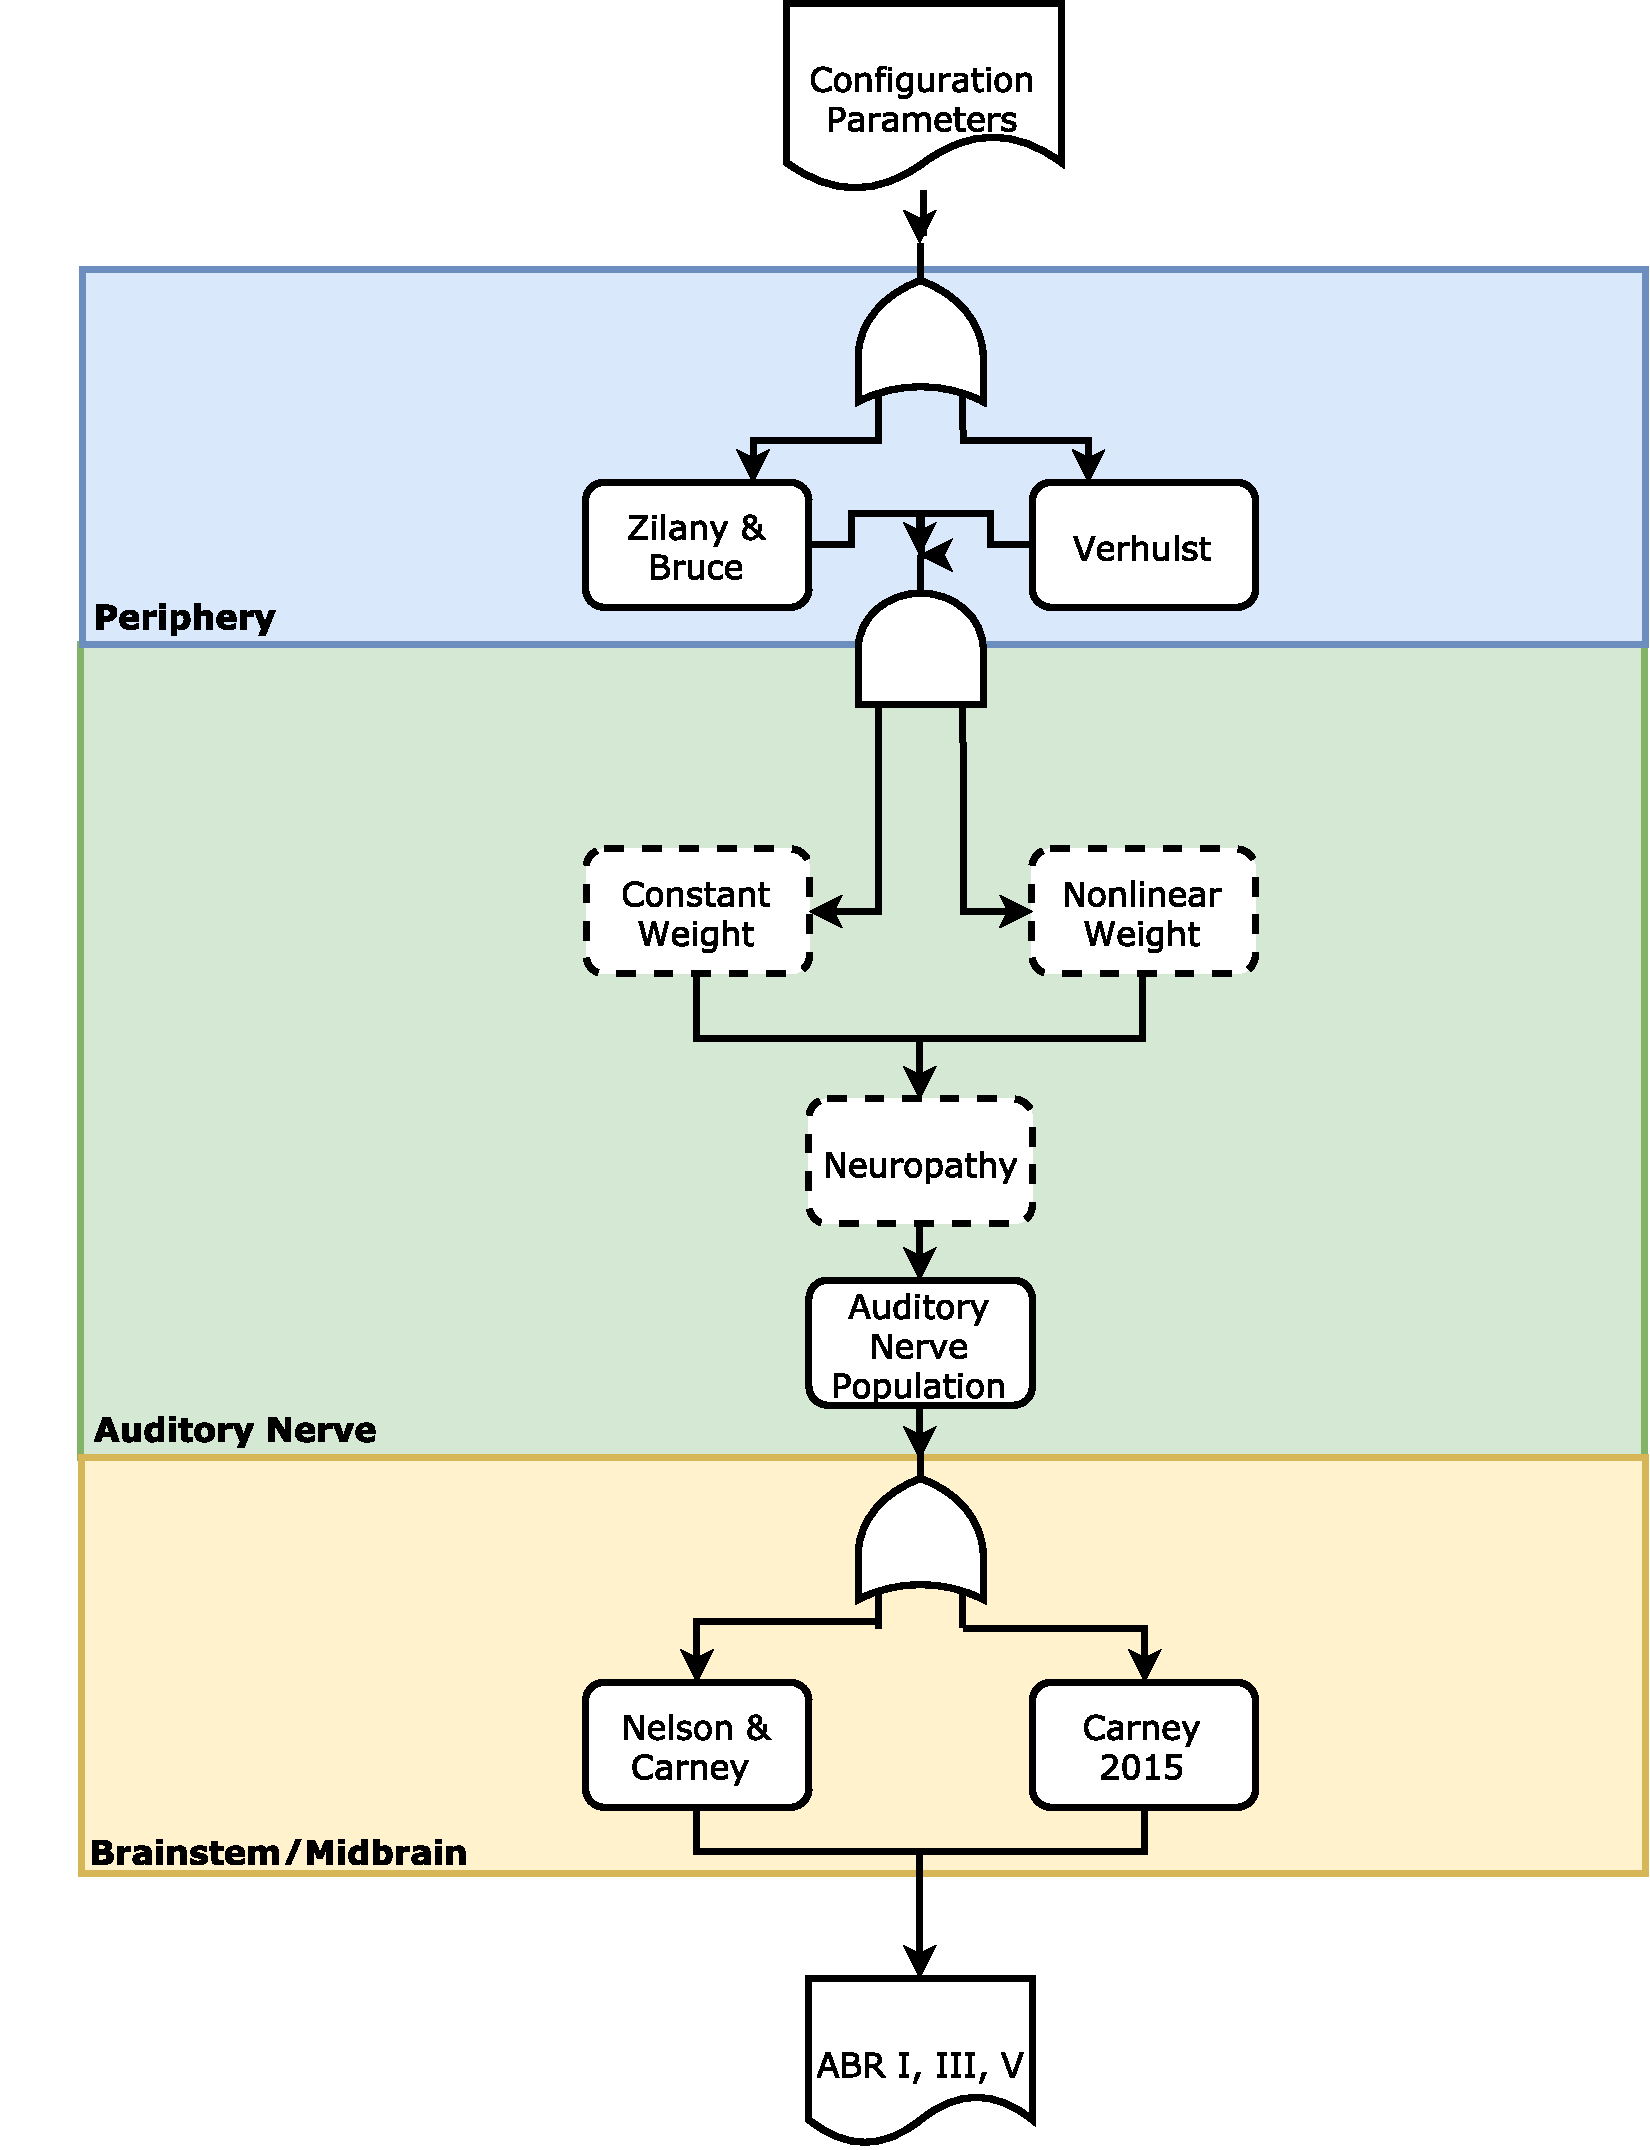
\includegraphics[width=0.95\textwidth]{high-level-overview.pdf}
	\caption[Overview of the Corti Modeling Environment.]{\textbf{Overview of the Corti modeling environment.}  In the Periphery region (blue), either the Zilany or Verhulst models produce estimates of IFRs for AN fibers from user-supplied stimuli.  In the Auditory Nerve region (green), IFR estimates for each AN fiber type are combined into the CAP.  In the Brainstem/Midbrain region (yellow), the CAP is convolved with CN and IC models to produce an ABR.}
	\label{fig:corti-overview}
	\end{figure}

\section{Simulation using Corti} % (fold)
\label{sec:simulation_using_corti}
As shown in \autoref{fig:corti-overview}, a full simulation using Corti involves three primary processing stages: the Peripheral, Auditory Nerve, and Brainstem / Midbrain. The next sections of this chapter will treat each stage in detail. 
% section simulation_using_corti (end)

\section{Peripheral Models} % (fold)
\label{sec:peripheral_models}
The Peripheral stage takes a stimulus and produces estimates of the Instantaneous Firing Rate for three fibers per CF.  Two models of the auditory periphery are included: the transmission-line model by~\cite{Verhulst2015Functional} (henceforth ``The Verhulst model'') and the phenomenological model by~\cite{Zilany2014Updated} (henceforth ``The Zilany model'').  This section corresponds to the first stage of \autoref{fig:corti-overview}, highlighted in blue.

As detailed in \autoref{fig:periphery-stage}, both the Verhulst and Zilany models simulate the response of the peripheral auditory system to a pressure wave, and both produce time-series estimates of Instantaneous Firing Rates (IFRs) for an arbitrary number of inner hair cells which are tonotopically distributed along the length of the basilar membrane via the Greenwood function.

\begin{figure}[htbp]
	\centering
	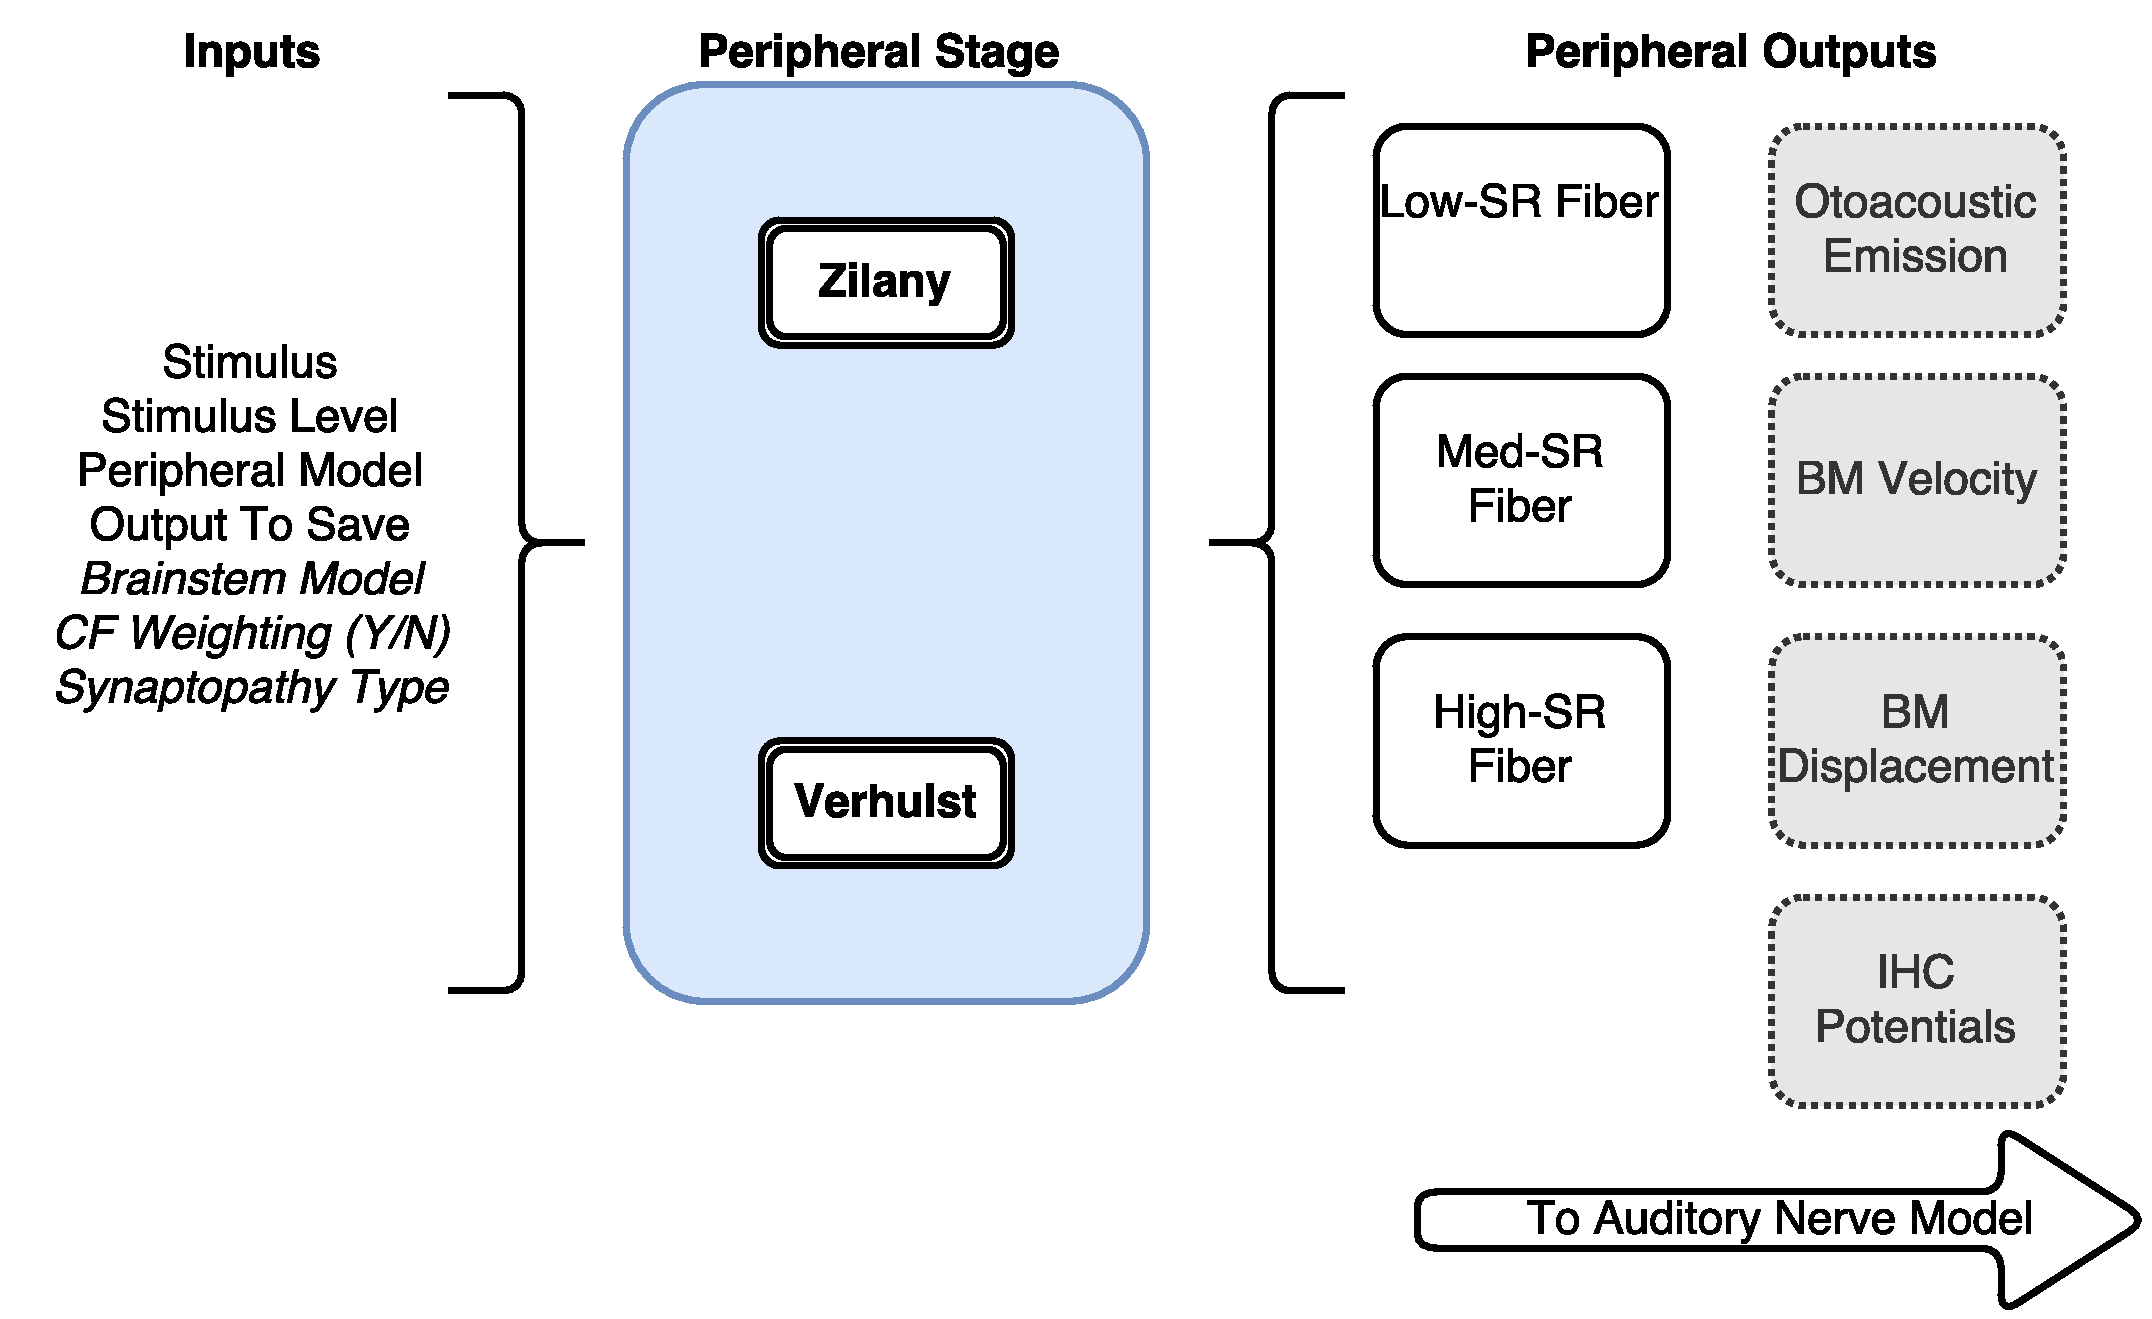
\includegraphics[width=0.95\textwidth]{periphery-subunit.pdf}
	\caption[The Peripheral Stage]{The Peripheral stage. All model inputs are shown; inputs in italics are used in later stages.  Three estimates of fiber IFRs are always produced (black bordered boxes) and are passed to the Auditory Nerve modeling stage.  The Verhulst model may also produce other output (grey dashed boxes) which can be optionally stored, but is not used for ABR estimation. }
	\label{fig:periphery-stage}
\end{figure}

\subsection{Accounting for Variations in Spontaneous Rates Between Models} % (fold)
\label{sub:interoperability_of_the_zilany_and_verhulst_models}
While both the Zilany and Verhulst models produce estimates of the instantaneous firing rate of the auditory nerve, the means by which they do so are different enough that care must be taken in directly comparing their estimates.  

The classification of SR types by mean spontaneous firing rate differs between the Zilany and Verhulst models.  The Zilany model defines a low-SR fiber to have a spontaneous rate of 0.1 spikes/second, a medium-SR fiber to have a spontaneous rate of 10 spikes/second, and a high-SR fiber to have a rate of 100 spikes/second.  The Verhulst model defines these values as 1, 10, and 60 spikes/second, respectively.  As discussed in \autoref{sub:low_spontaneous_rate_fibers_suffer_selective_losses} and \autoref{sub:weighting_of_fiber_types_per_ihc}, \cite{Temchin2008Threshold} combine low- and medium-SR fibers into one population and define it to have a spontaneous rate of less than 18 spikes/second.  For the purposes of this work, both the Zilany and Verhulst model support this approach.  

Therefore, while both the Verhulst and Zilany model support classification of spontaneous rates into three categories, for the purposes of weighting fiber types both low- and medium-SR populations may be treated identically.  

\subsection{Weighting of IHC contributions} % (fold)
\label{sub:weighting_of_ihc_contribution}
To determine which proportion of the total contribution of a given hair cell arises from fibers of a given spontaneous rate, the Verhulst model applies a scalar weighting factor to the summed Auditory Nerve Response using an undamaged nerve with 19 total fibers. Three fibers are assigned for low- and medium- SR fibers and 13 for high-SR fibers per hair cell. 

Once each hair cell's contribution has been computed and summed into the total response,  a scalar weighting factor was empirically chosen such that the modeled and summed response of IHCs with CFs between 175Hz and 20kHz produces a model ABR Wave I amplitude of 15 $\mu$V.  For the Verhulst model, \cite{Verhulst2015Functional} found the value of this weighting factor to be \num{0.15e-6} V $\times$ \num{2.7676e-07}.  This weighting factor is given as a product to emphasize that it directly fixes the peak Wave I output at 15$\mu$V. 

To produce comparable results in this work, the Zilany model was scaled accordingly. We iteratively converged on a scaling factor that produced an ABR Wave I amplitude of 15$\mu$V$\pm 1$nV, which was found to be \num{0.15e-6} V $\times$ \num{7.30282e-07}.
% subsection weighting_of_ihc_contribution (end)


\subsection{The Verhulst Model} % (fold)
\label{sub:the_verhulst_model1}
The Verhulst model is particularly well-suited for modeling broadband stimuli.  Since it is a transmission line model which gives estimates for the position and deflection of the entire basilar membrane even to a pure tone stimulus, it naturally accounts for dispersive effects, and produces detailed information about many stages of sound propagation. Though not used in this work, the Verhulst model is also capable of modeling Otoacoustic emissions in response to complex stimuli. 

Since the development of the Verhulst model is still underway by Verhulst et.~al., it has been programmatically isolated in a separate package.  This provides a separation of concerns between the projects, and allows both Corti the modeling framework, and the Verhulst model itself to be updated independently of each other as new features are made available in both.
% subsection the_verhulst_model (end)
\subsection{The Zilany Model} % (fold)
\label{sub:the_zilany_model}
The Zilany model is a very commonly used model of the auditory periphery, and robustly accounts for many phenomena observed electrophysiologically to complex stimuli.  The model was originally developed based on measurements in cat \citep{Zilany2006Modeling},and has since been updated to account for spectrally complex sounds via power-law adaptation \citep{Zilany2007Predictions} and later with humanized parameters to better reflect psychophysical data \citep{Zilany2014Updated}. 

The implementation of the Zilany model here was adapted from~\cite{Rudnicki2014Cochlea}, who provided a Python and C implementation that has been shown to produce identical output to the version documented by~\cite{Zilany2014Updated}.


% subsection the_zilany_model (end)

\subsection{Peripheral Model Output} % (fold)
\label{sub:peripheral_model_output}
The Verhulst model provides estimates of response behavior at many stages of the of the auditory periphery.   For models of motion in the middle ear, estimates are computed for each basilar membrane section.  By default, the BM is divided into 1000 section.  Each section corresponds to one CF, where the place-frequency map is obtained via the Greenwood function.

 While running the simulation, the following model outputs may be stored to disk for further analysis: 
\begin{enumerate}
	\item Basilar membrane velocities for each section.
	\item Basilar membrane displacements for each section.
	\item Inner hair cell receptor potentials. 
	\item IFR for a high spontaneous rate fiber.
	\item IFR for a medium spontaneous rate fiber.
	\item IFR for a low spontaneous rate fiber. 
	\item The Otoacoustic emission. 
\end{enumerate}

The Zilany model, as implemented, provides IFR estimates only.  Hair cell potentials could also be modeled, but are omitted.

Both models provide estimates of Instantaneous Firing Rate as a function of post-stimulus time for each combination of fiber type and best frequency, and these are passed to the next stage of the Corti environment.
% subsection peripheral_model_output (end)

% section peripheral_models (end)

\section{Auditory Nerve Response Models} % (fold)
\label{sec:auditory_nerve_response_models}
This stage of processing converts IFRs of specific fiber populations made by either the Zilany or Verhulst model into an estimate of the summed activity of the auditory nerve. It corresponds to the green-shaded region of \autoref{fig:corti-overview}, and is outlined in detail in \autoref{fig:an-subunit}.  Depending on the parameters chosen, output of either the Zilany or Verhulst peripheral models are first summed into a population response of the AN by one of two means.  Next, degradation of the population response that corresponds to a model of synaptopathy is applied; finally, the summed population response is passed to the midbrain and brainstem models.

\begin{figure}[htbp]
	\centering
	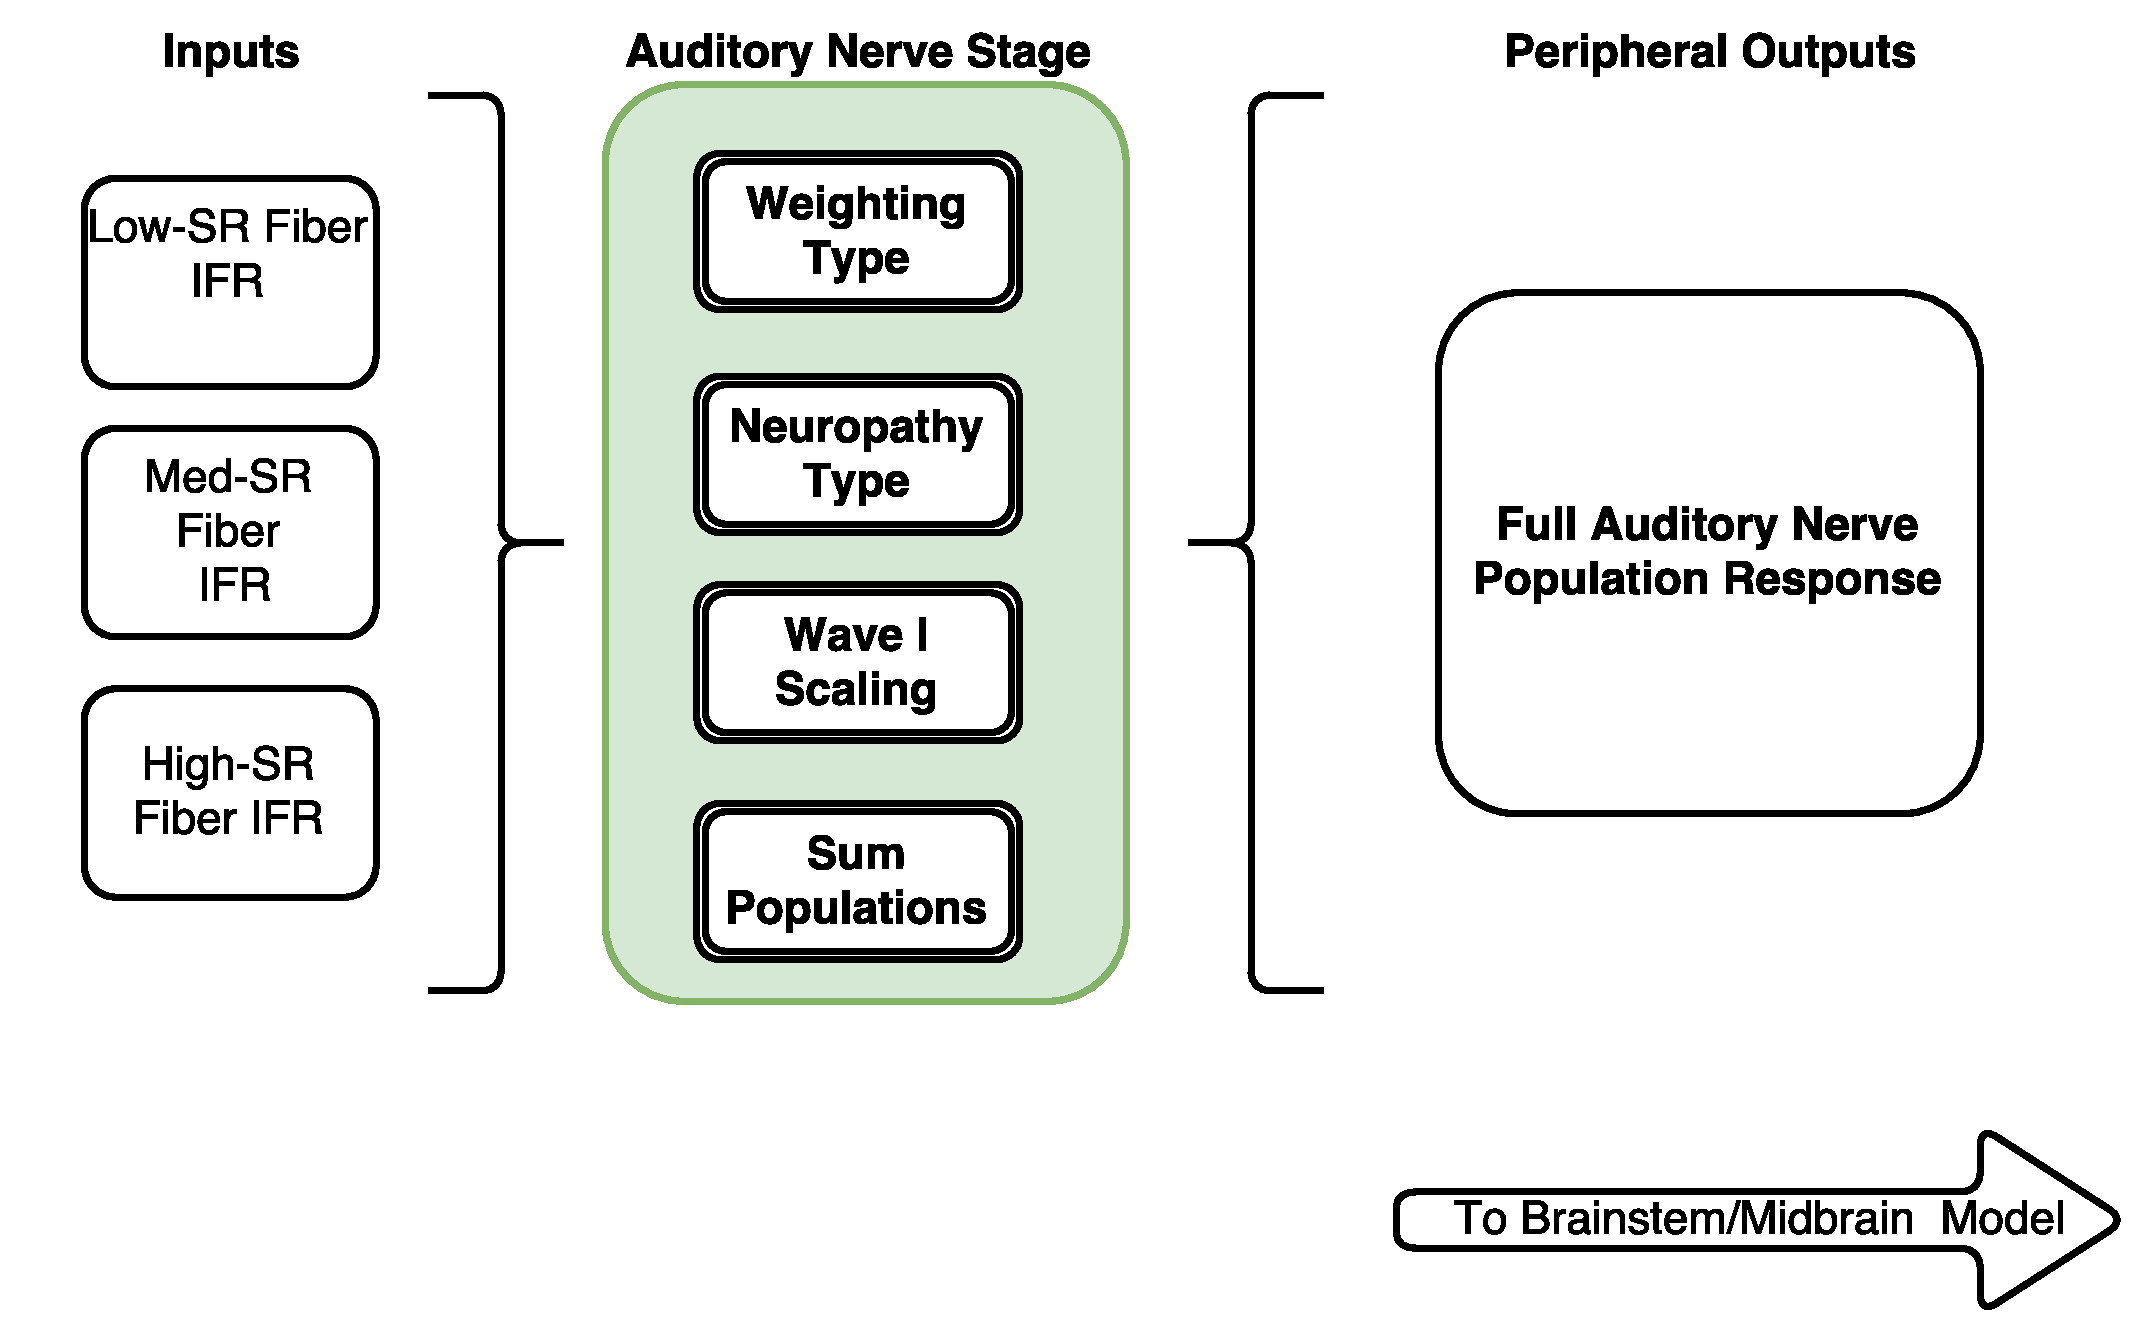
\includegraphics[width=0.95\textwidth]{an-subunit.pdf}
	\caption[The Auditory Nerve Stage]{The Auditory Nerve Stage. Single IFR estimates for fiber types at each CF are weighted to produce an estimate of the total IFR at each IHC/CF.  These are optionally degraded to model synaptopathy, weighted to produce physiologically appropriate Wave I amplitudes, and summed into the total population response of the Auditory Nerve.}
	\label{fig:an-subunit}
\end{figure}

\subsection{Modeling the Contributions of Inner Hair Cells} % (fold)
\label{sub:contributions_to_the_response_by_inner_hair_cells}
The output of the Zilany and Verhulst peripheral models are IFRs for one stereotypical AN fiber of each SR type per CF.   However, tens of fibers synapse on each IHC along the length of the cochlea.  Consequently, to generate an estimate of IFR per CF or per BM section, each stereotypical AN fiber must be scaled by some weighting factor so that its output becomes an estimate of the summed IFRs of its SR category for a given IHC.  Based on anatomical data \citep{Liberman1978AuditoryNerve}, the Verhulst model assigns 19 fibers to each inner hair cell.  The Zilany model makes no inherent assumptions about the number of fibers per IHC. To maintain equivalence with the Verhulst model and allow like-to-like comparison of model output, IFR estimates from both models are distributed among 19 fibers.

In \autoref{fig:corti-overview}, this process is the first contribution of the AN processing area in green, and is accomplished by either a constant or nonlinear weight.

% subsection contributions_to_the_response_by_inner_hair_cells (end)


\subsection{Weighting of Fiber Types per IHC} % (fold)
\label{sub:weighting_of_fiber_types_per_ihc}
Based on data from~\cite{Temchin2008Threshold}, and as reviewed in \autoref{sec:physiology_of_the_auditory_nerve}, the distribution of SR fiber types per IHC may not be uniform along the length of the basilar membrane.  To account for this, we have extended the linear distribution of fiber types per hair cell with the option of a logistic distribution as a parameter.   As shown in \autoref{fig:temchin-curvefit}, experimental data for SR distribution as a function of CF was fitted via logistic regression in \textsc{matlab}, and this regression function was used to generate an empirical estimate of SR type. 

\begin{figure}[htbp]
	\centering
	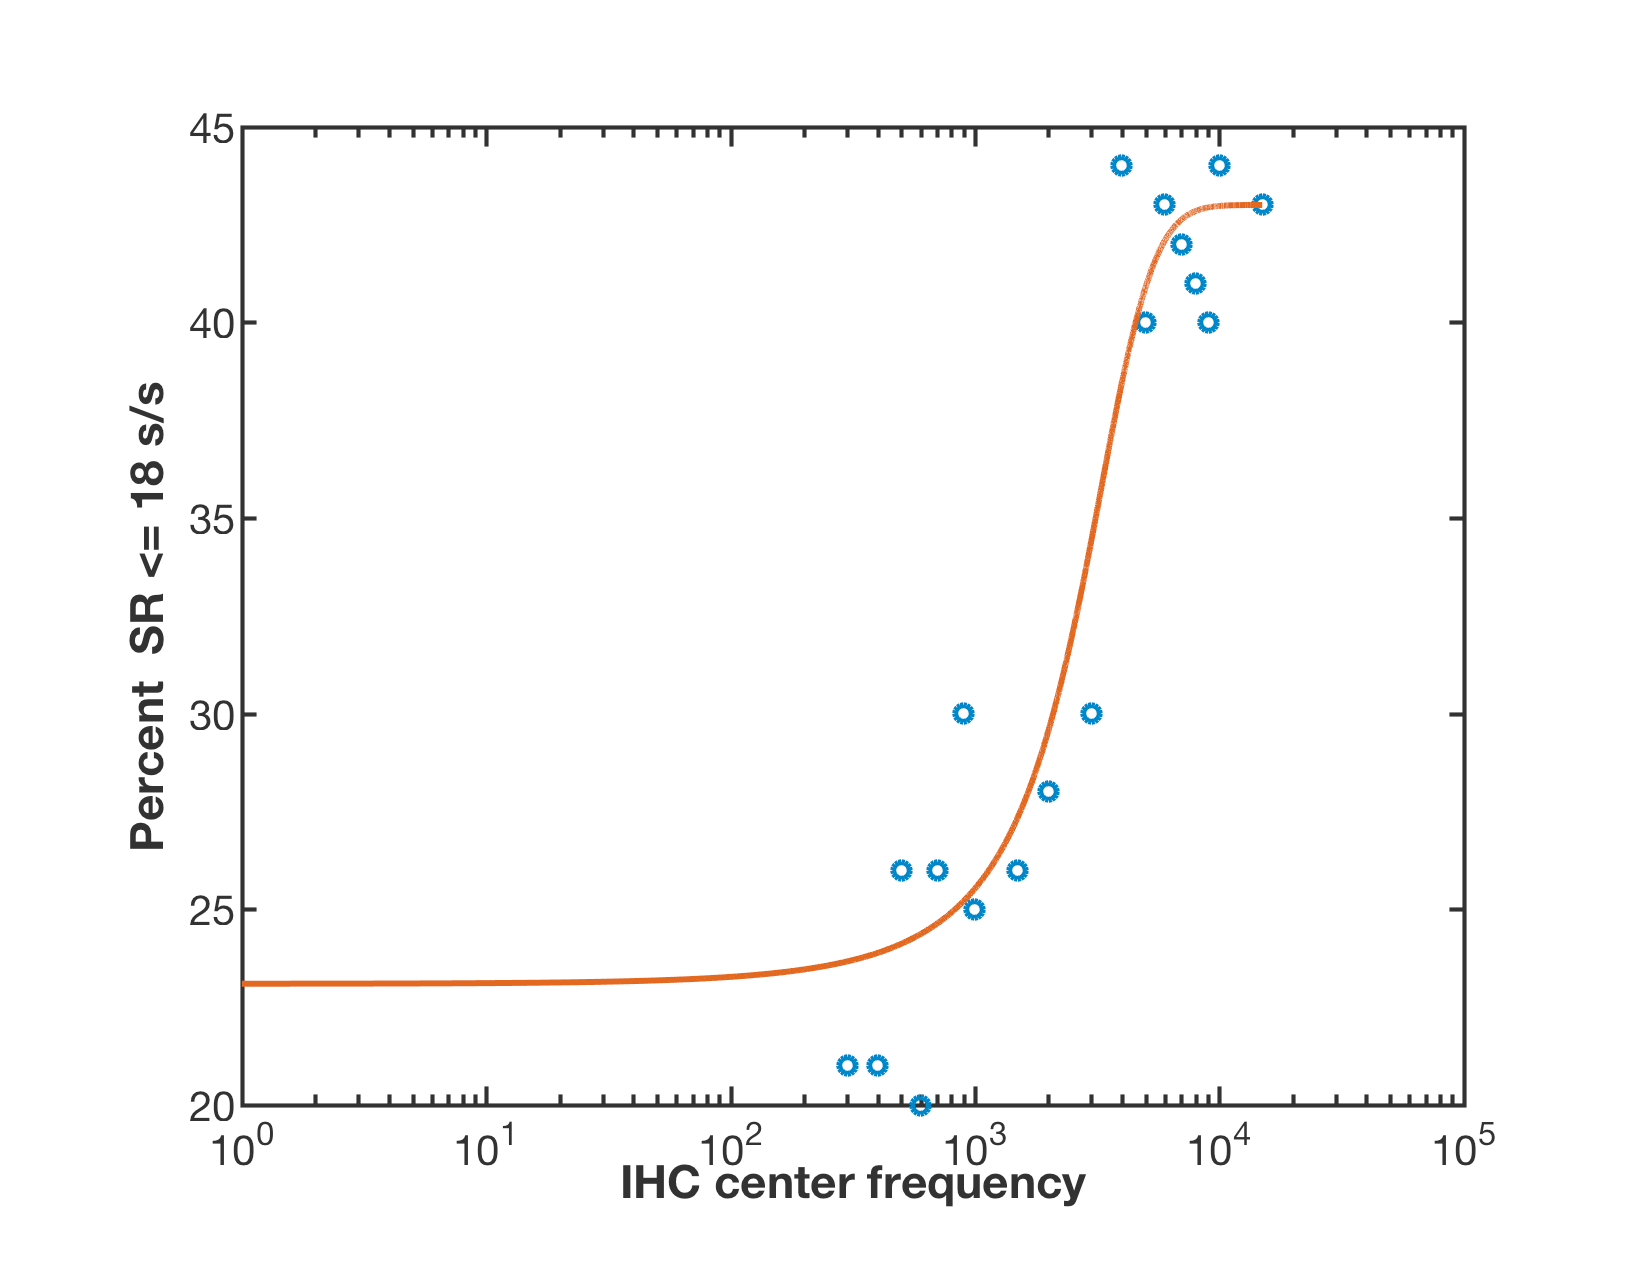
\includegraphics[width=0.95\textwidth]{temchin-curvefit.pdf}
	\caption[Variation in Spontaneous Rate as a Function of Frequency]{Experimental results (blue circles) reported by \cite{Temchin2008Threshold} were fit to a logistic model (red solid line).}
	\label{fig:temchin-curvefit}
\end{figure}

The empirical logistic fit equation that estimates $p$, the percentage of fibers with spontaneous rates below 18 spikes/sec innervating a given inner hair cell as a function of best frequency was found to be: 

\begin{equation}
	p(\mathit{cf}) = 21 + \frac{k}{1+e^{-r\cdot(\mathit{cf}-\mathit{cf}_0)}}
\end{equation}

where $k = 22$, $r = $ \num{9e-6} and $\mathit{cf}_0 = 2500$.

\subsubsection{Fractional Weights}
A consequence of the IFR weighting approach taken here is that while the total fiber count per IHC is fixed at 19 fibers, the percentage of the summed response of that IHC that arises from a given fiber type is not guaranteed to represent an integer number of fibers.  For example, a CF of 8 kHz has 42.9 percent of its innervating spiral ganglia with spontaneous rates below 18 spikes/second, or a total of 8.133 low and medium spontaneous rate fibers.  

Therefore, it is appropriate to think of the modeled IFR values as the weighted contributions of a SR type to the overall IFR originating from a particular CF, rather than the summed responses of integer numbers of individual fibers.  In the context of producing auditory nerve responses---as are used in this work---this can be thought of as providing a more accurate representation of \emph{summed} physiological responses. Model responses of unitary fibers of different spontaneous rates are saved in the peripheral output, if desired.
% subsection weighting_of_fiber_types_per_ihc (end)

\subsection{Modeling Synaptopathy} % (fold)
\label{sub:modeling_synaptopathy}
Cochlear synaptopathy is the loss of the synapse between an inner hair cell and an individual spiral ganglion.  At the level of the summed auditory nerve response, selective degradation is modeled by reducing the contribution of each fiber type per hair cell by a scaling factor. 

Six predetermined severity levels, as given in \autoref{fig:synaptopathy} were chosen to model cochlear synaptopathy, all of which behave similarly.  In each case, the portion of the response from a hair cell of a given center frequency is scaled by a percentage of its magnitude before being summed into the auditory nerve response.  

\begin{figure}[htbp]
	\centering
	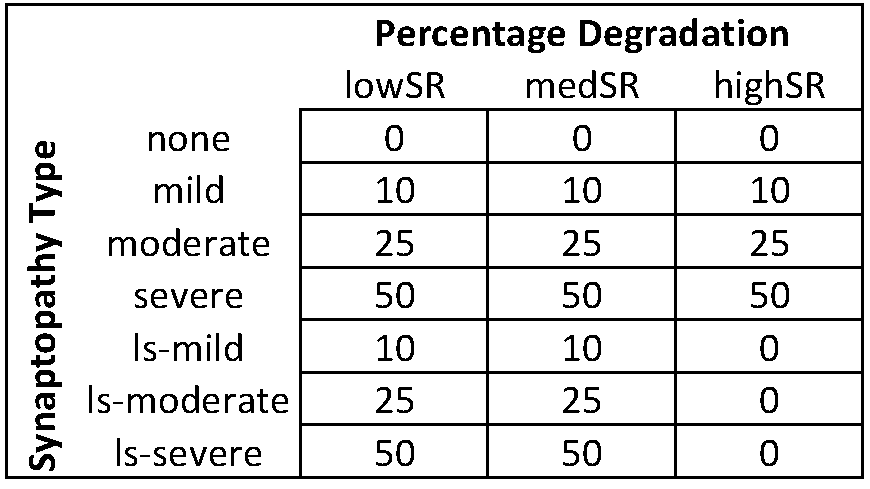
\includegraphics[width=0.95\textwidth]{percentage-degradation.pdf}
	\caption[Cochlear Synaptopathy Parameters]{The default types of cochlear synaptopathy that may be simulated. The percentage by which the IFRs of a given fiber type are reduced are given in each row.  In the case of the Low SR (ls) synaptopathies ls-mild, ls-moderate, and ls-severe, only the low- and medium- SR fibers are degraded.}
	\label{fig:synaptopathy}
\end{figure}
% subsection modeling_synaptopathy (end)
% section auditory_nerve_response_models (end)

\section{Brainstem Models} % (fold)
\label{sec:brainstem_models}
This section details the two brainstem models in use, given by~\cite{Nelson2004Phenomenological} and~\cite{Carney2015Speech}.  These correspond to the yellow region of \autoref{fig:corti-overview}, and are detailed in \autoref{fig:brainstem-subunit}.

\begin{figure}[htbp]
	\centering
	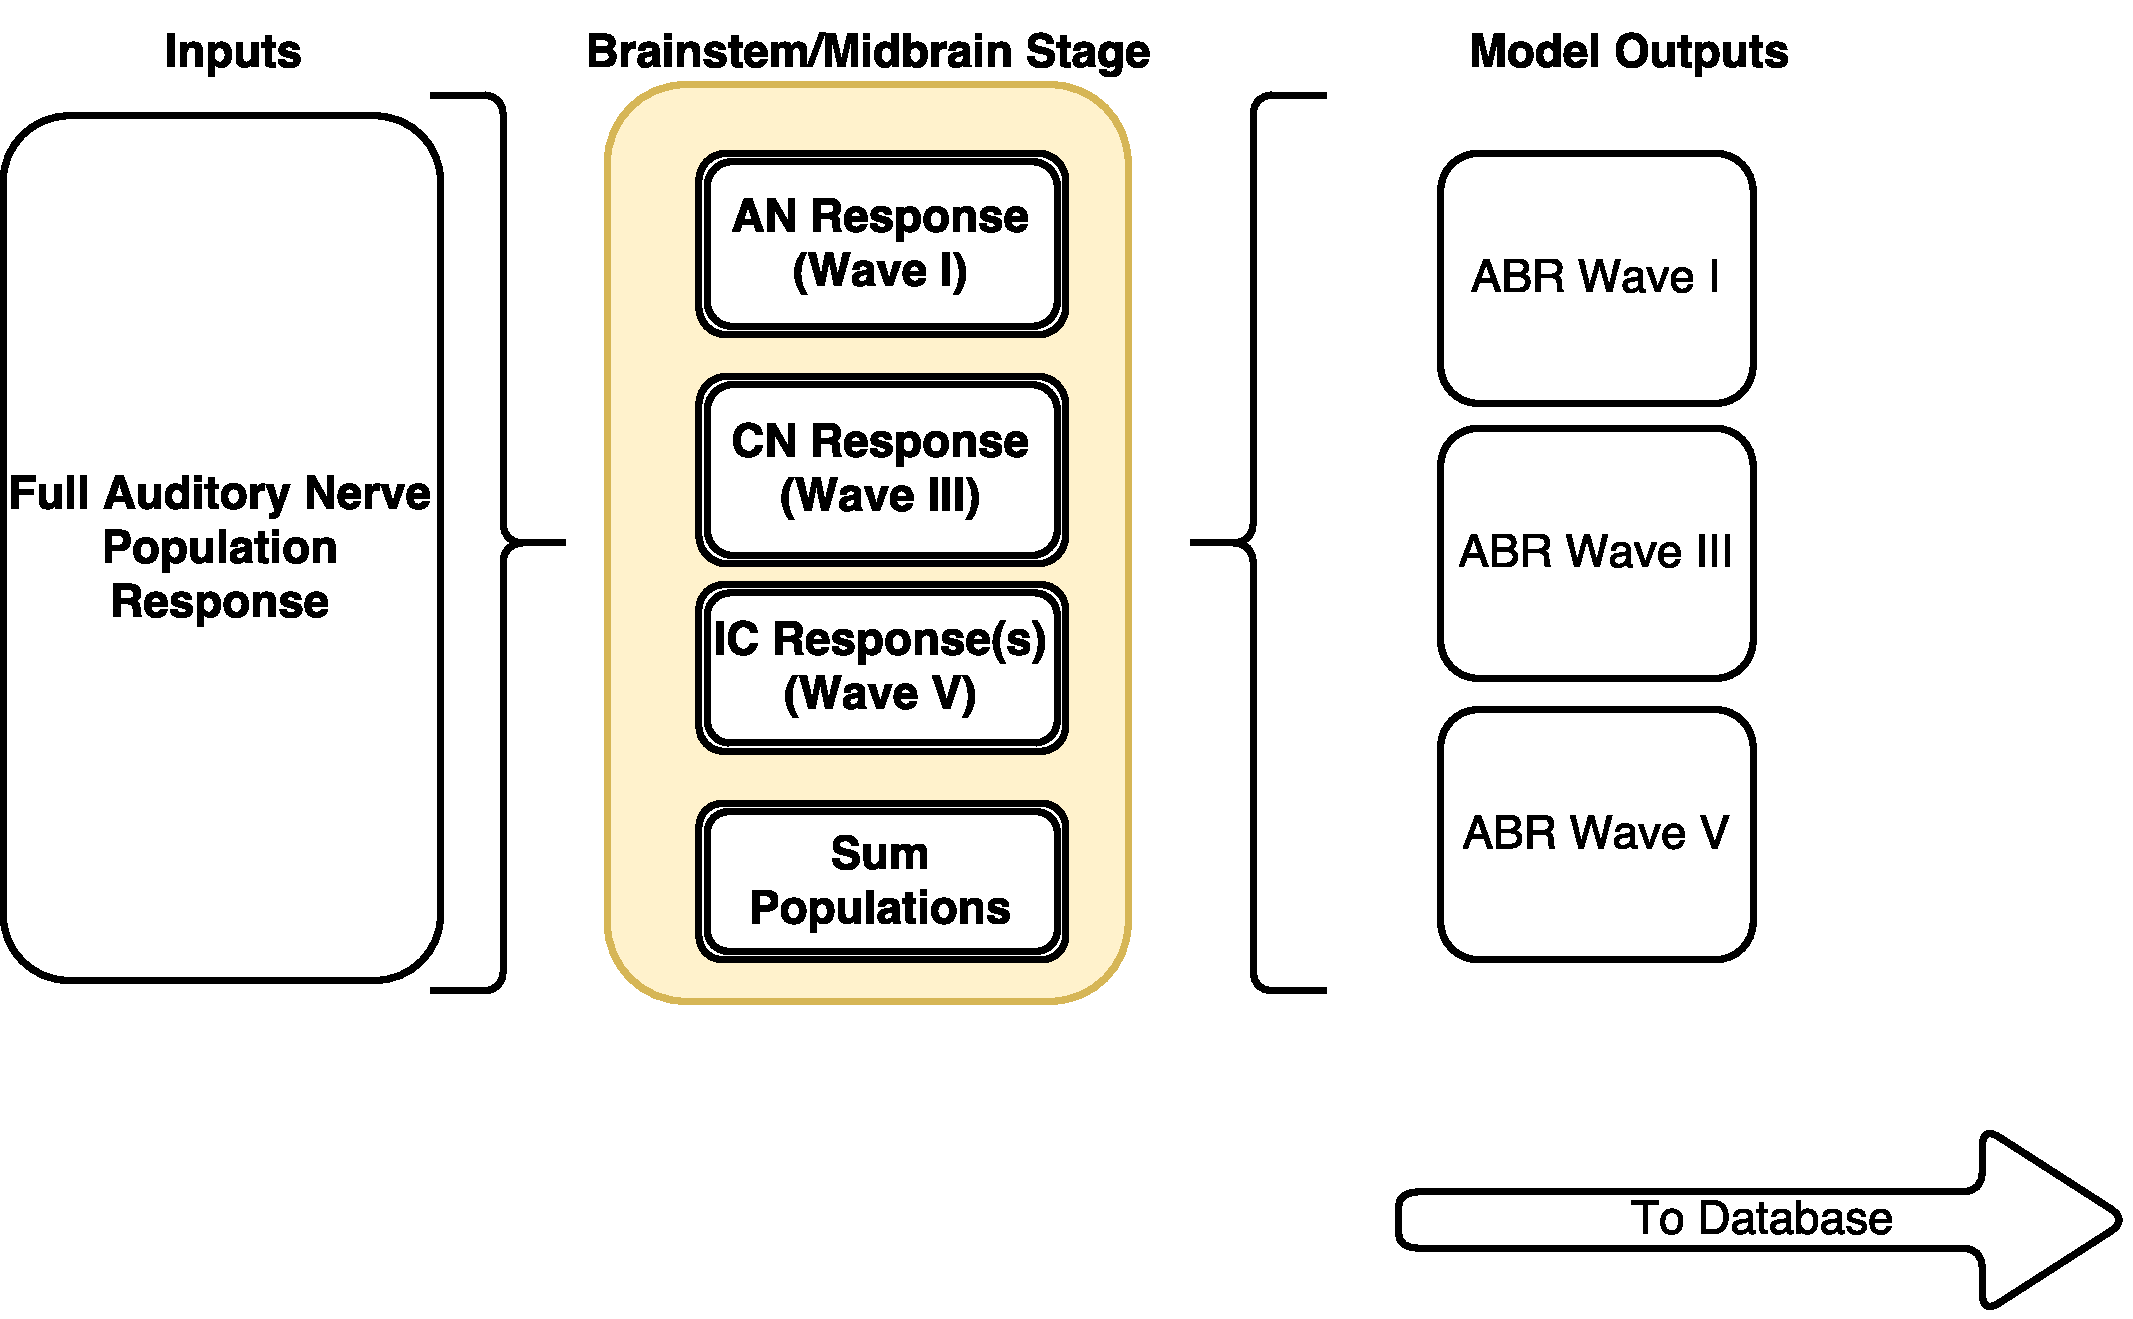
\includegraphics[width=0.95\textwidth]{brainstem-subunit.pdf}
	\caption[The Brainstem and Midbrain Stage]{The Brainstem and Midbrain stage.  The summed Auditory Nerve population response is convolved with Same-Frequency Inhibition/Excitation models to produce estimates of the Cochlear Nucleus response.  Wave I estimates are made from the AN response.  The response of the IC is simulated with one or three SFIE model(s), depending on which brainstem model was chosen.  From the CN and IC responses, estimates of Waves III and V are made.}
	\label{fig:brainstem-subunit}
\end{figure}

\subsection{Choice of Best Modulation Frequency}
The included models of the CN and IC are tuned to a best modulation frequency (BMF)---i.e., the stimulus modulation frequency at which they have a peak response---of 100 Hz, as this was found by~\cite{Carney2015Speech} to be the most relevant modulation frequency for speech-like complex sounds such as vowel formants. These responses thus may be regarded as Modulation Transfer Functions (MTF).  It is not clear the extent to which the CN or IC possess a ``MTF filter-bank'', where units are tuned to multiple BMFs, so this has not been implemented.

\subsection{The Nelson Carney 2004 Brainstem} % (fold)
In the case of the simpler brainstem and midbrain model of \cite{Nelson2004Phenomenological}, the CN and IC are both represented as single processing stages where an excitatory and inhibitory alpha function are convolved with, in the CN, the ANR population response, and in the IC, the output of the CN stage. 
\label{sub:the_nelson_carney_2004_brainstem}
\begin{figure}[htbp]
	\centering
	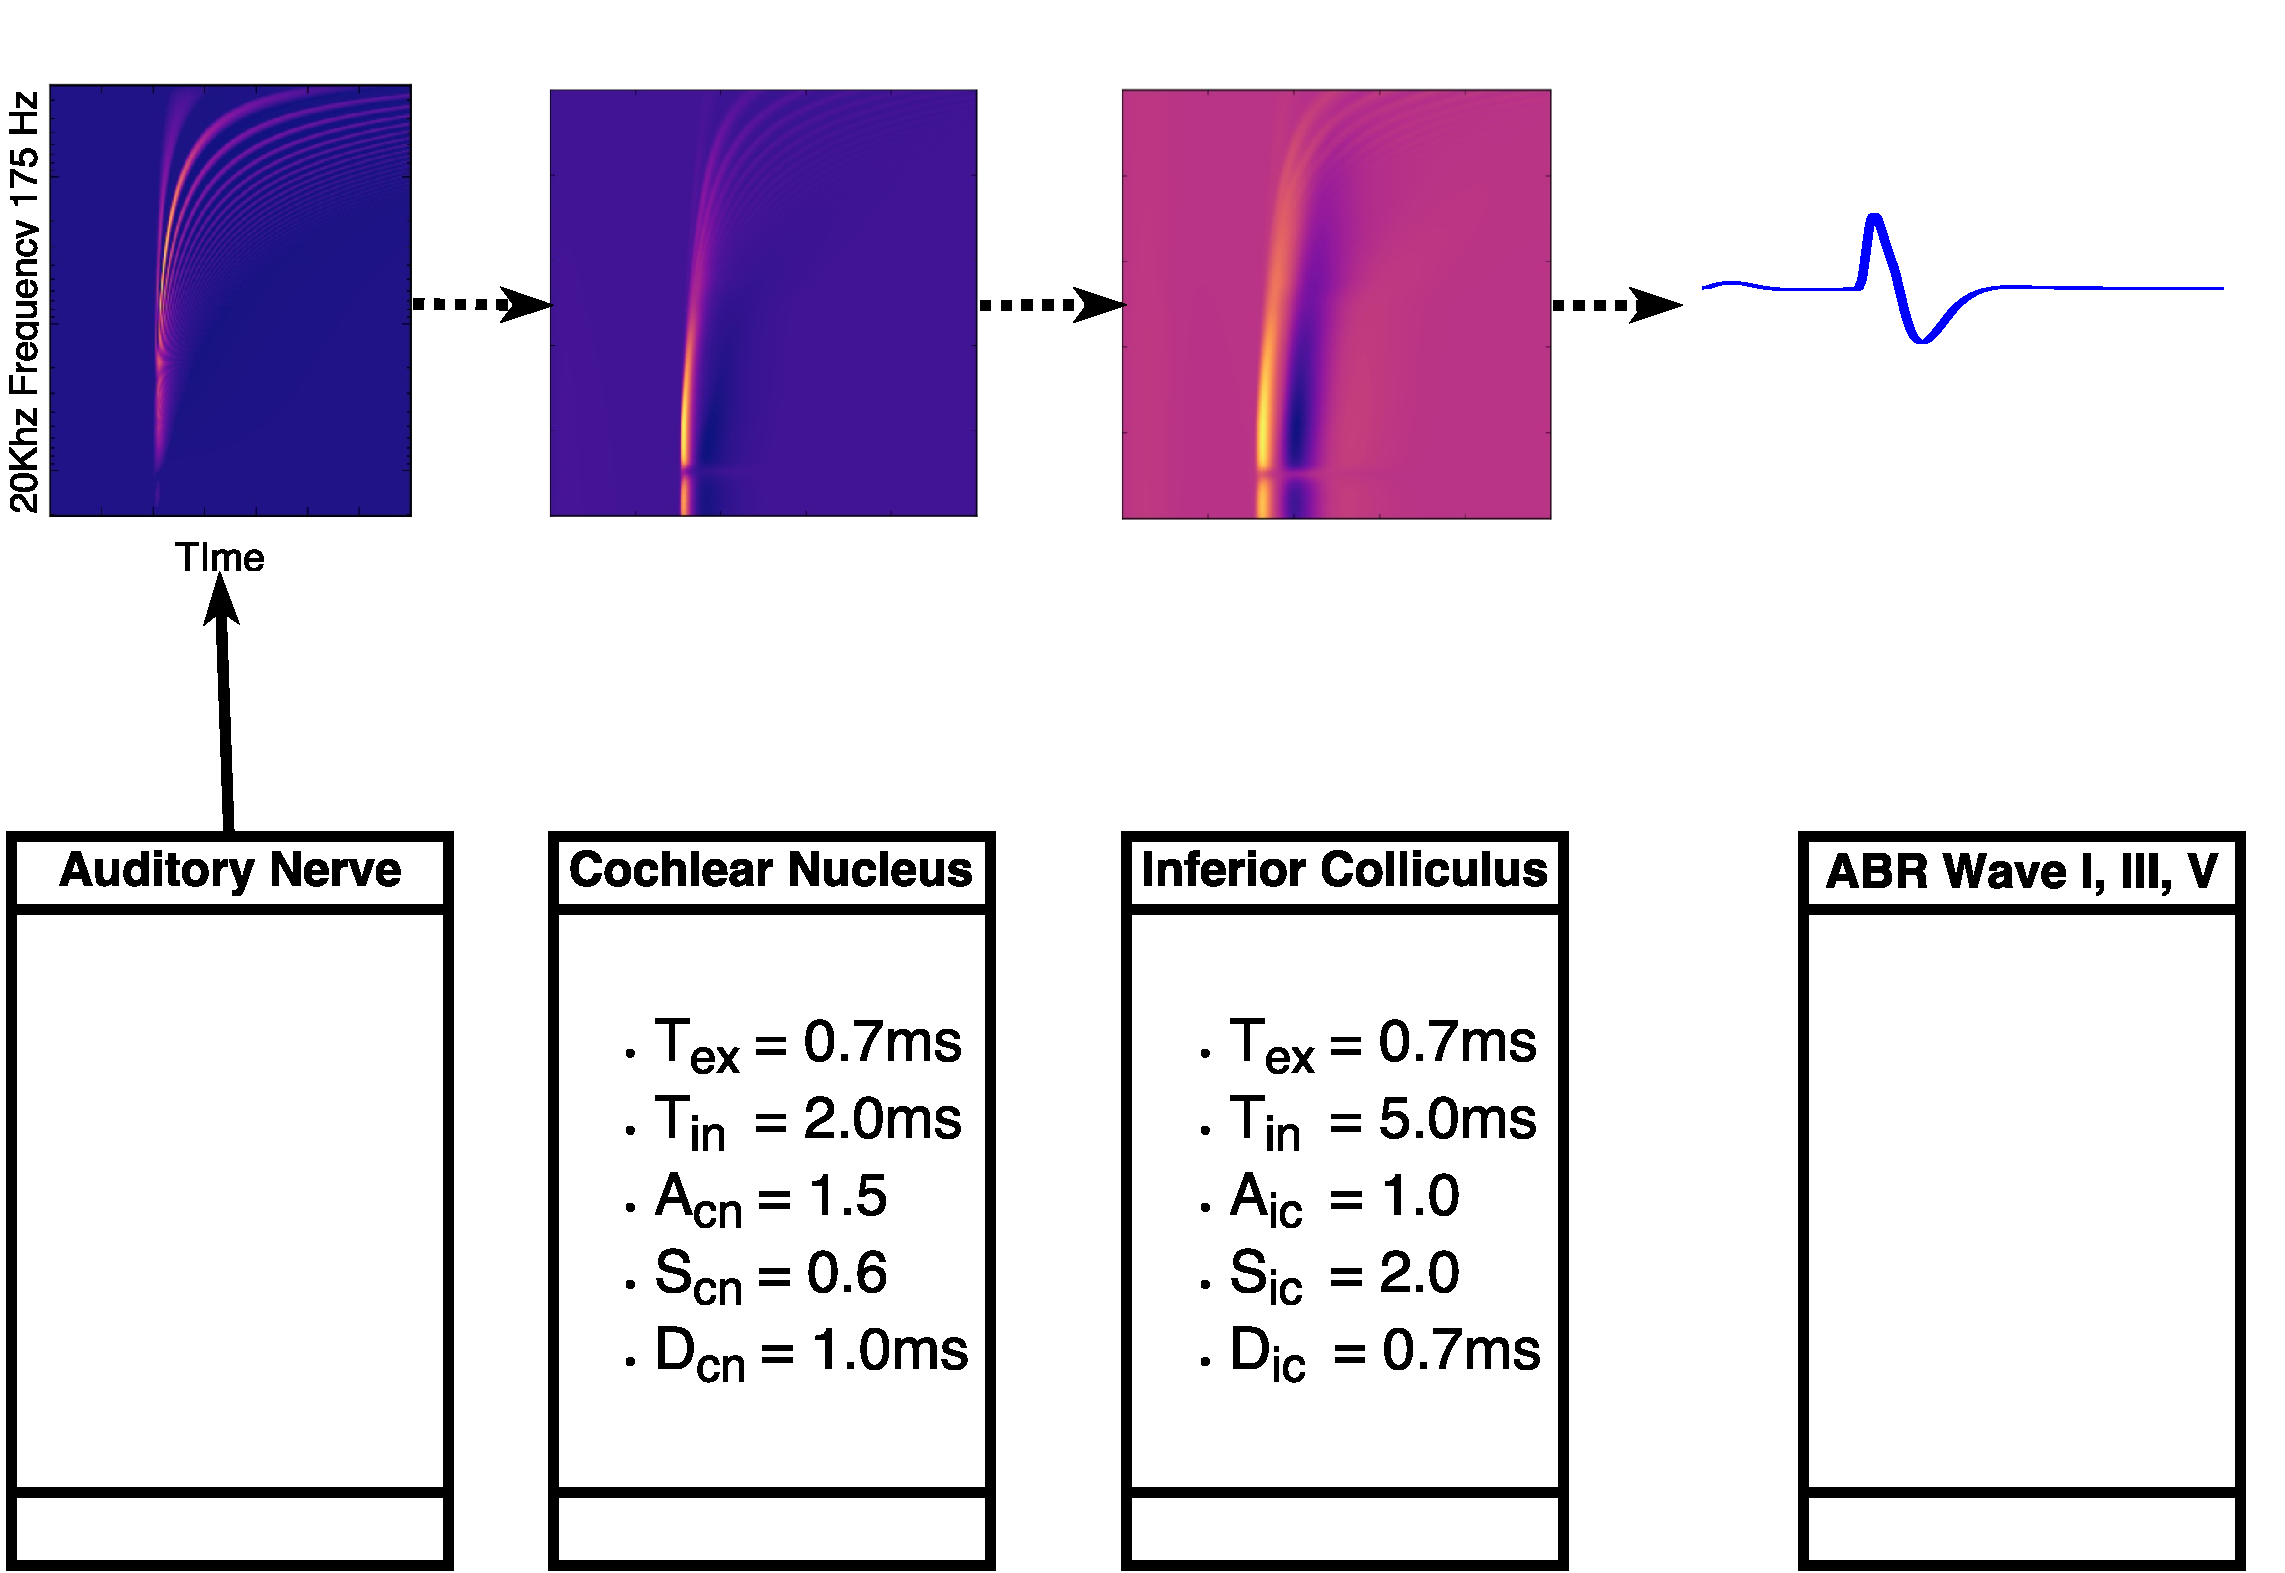
\includegraphics[width=0.95\textwidth]{nelson-carney-2004.pdf}
	\caption[Overview of the Nelson-Carney Midbrain and Brainstem]{Overview of the processing stages of the Nelson-Carney brainstem model and model output at various stages for an 80dB click stimulus. Coefficients, which define the excitation and inhibition onset times and amplitudes for the CN and IC, are given. }
	\label{fig:nelson-carney}
\end{figure}
% subsection the_nelson_carney_2004_brainstem (end)
\subsection{The Carney 2015 Brainstem} % (fold)
\label{sub:the_carney_2015_brainstem}
In the case of the more complex model proposed by \cite{Carney2015Speech}, the IC processing stage incorporates three types of filters, which better reflect the diversity of neural responses observed electrophysiologically. 

Weights of contribution for each type are as shown in \autoref{fig:carney-2015}, and were chosen to represent the relative magnitudes of effect observed by~\cite{Carney2015Speech} in electrophysiological study.  Weighing is uniform across center frequency.

\begin{figure}[htbp]
	\centering
	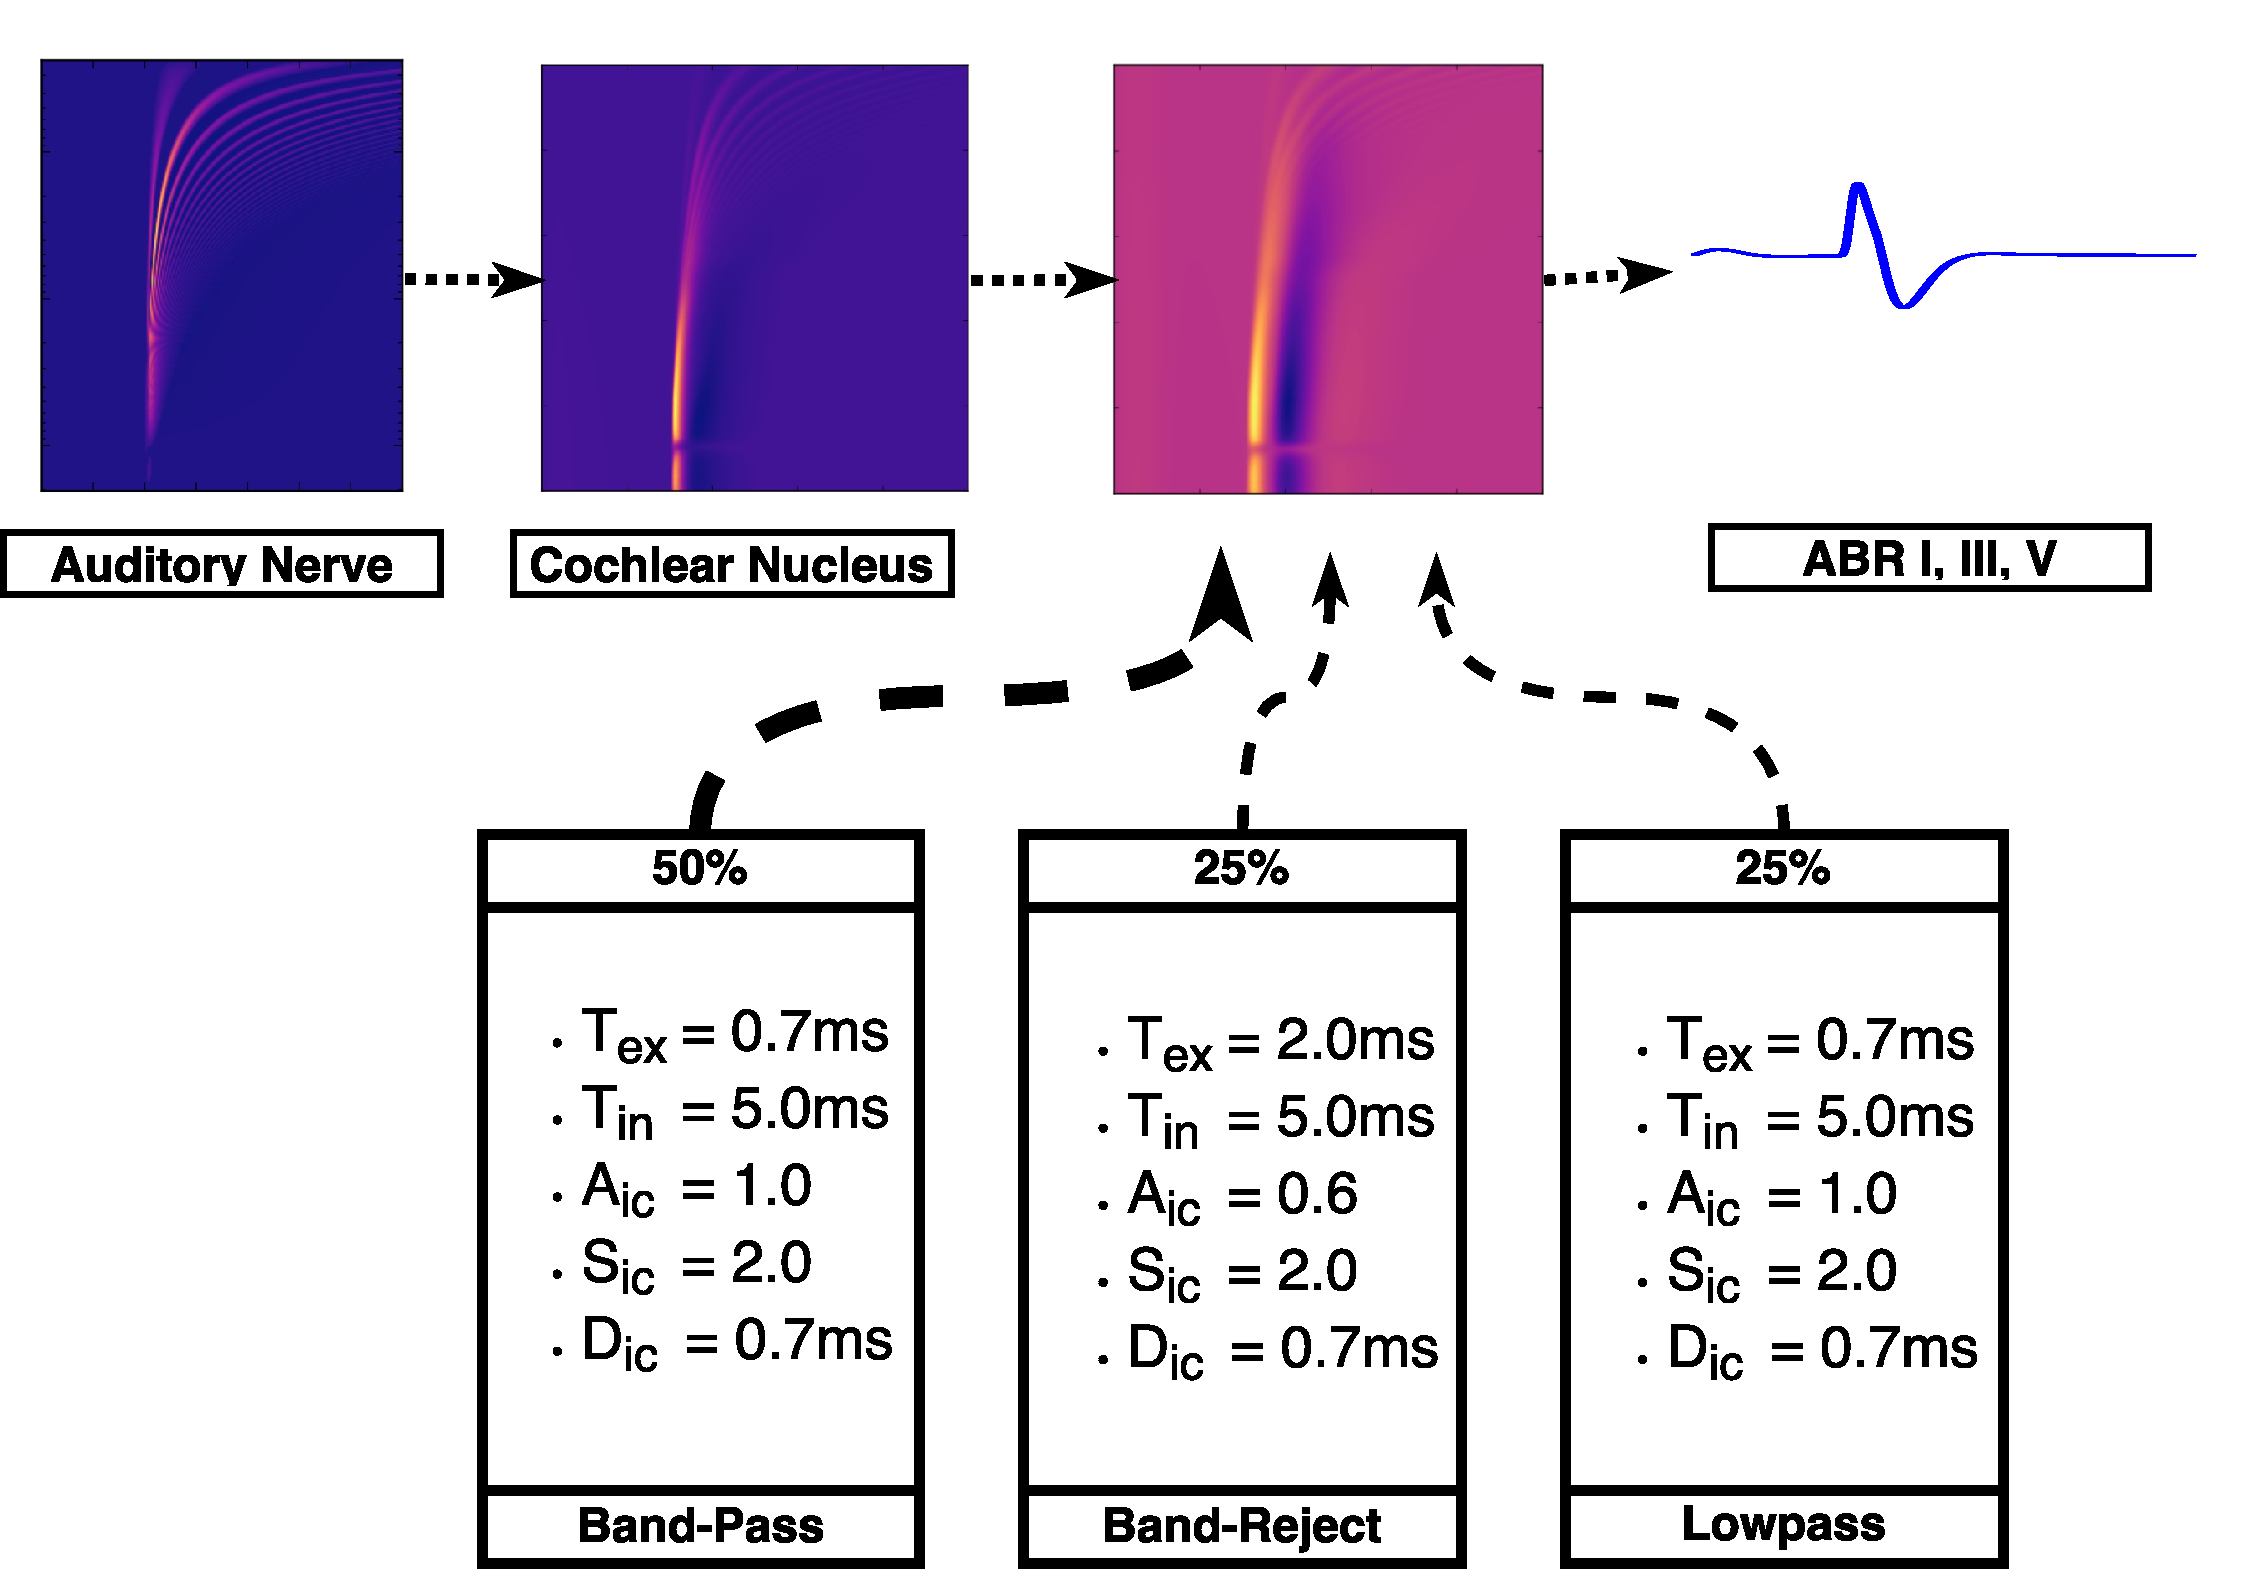
\includegraphics[width=0.95\textwidth]{carney-2015.pdf}
	\caption[Overview of the Carney Midbrain and Brainstem]{Overview of the processing stages of the~\cite{Carney2015Speech} brainstem model for an 80dB click.  Coefficients and weights for the three-stage IC model are shown; other parameters are as in \autoref{fig:nelson-carney}}
	\label{fig:carney-2015}
\end{figure}


% subsection the_carney_2015_brainstem (end)
% section brainstem_models (end)
\section{Stimulus Generation} % (fold)
\label{sec:stimulus_generation}
Corti supports simulations of stimuli of arbitrary duration and level.  Simple stimuli such as clicks are generated programmatically by specifying a series of parameters such as onset time and duration.  

More complex stimuli can be created and passed in as WAV files.  All WAV stimuli must specify the sound level, in dB SPL re 20$\mu$Pa, at which they should be presented; the waveform is then normalized by the peak value (in the case of a click) or the RMS value (for spectrally complex stimuli) and rescaled to have units of Pascals prior to simulation.
% section stimulus_generation (end)
\section{Automated Parameter Exploration} % (fold)
\label{sec:automated_parameter_exploration}
Corti may be run in one of two modes.  In the first, a single set of parameters defines a single trajectory and the model is run once.   However, while this mode of operation is convenient for fast simulations whose parameters can be defined \emph{a priori}, it rapidly becomes impractical for situations where the relative effects of different parameter choices are to be compared, and reliable book-keeping of which parameters were used to generate which results becomes unnecessarily challenging.

Therefore, a second means of use was created, as detailed in \autoref{fig:pypet-overview}. The core of this mode is the Python Parameter Exploration Toolkit \citep{Meyer2016Pypet}. It provides the tools to allow a convenient interface to explore the parameter space generated by the specification of many available models, impairments, and options in a manner that allows easy \emph{post-hoc} analysis. Individual trajectories may be computed in parallel on a single workstation or in a high-performance cluster so that the relative effects of each model, neuropathic impairment, and other features may be directly compared.  The results for all combinations of model components are stored in one Hierarchical Data Format (HDF5) file.  Comparisons of the effect of using different trajectories to the same stimuli (cross parameter differences) can then be made in a way that guarantees an internally consistent analysis.

\begin{figure}[htbp]
	\centering
	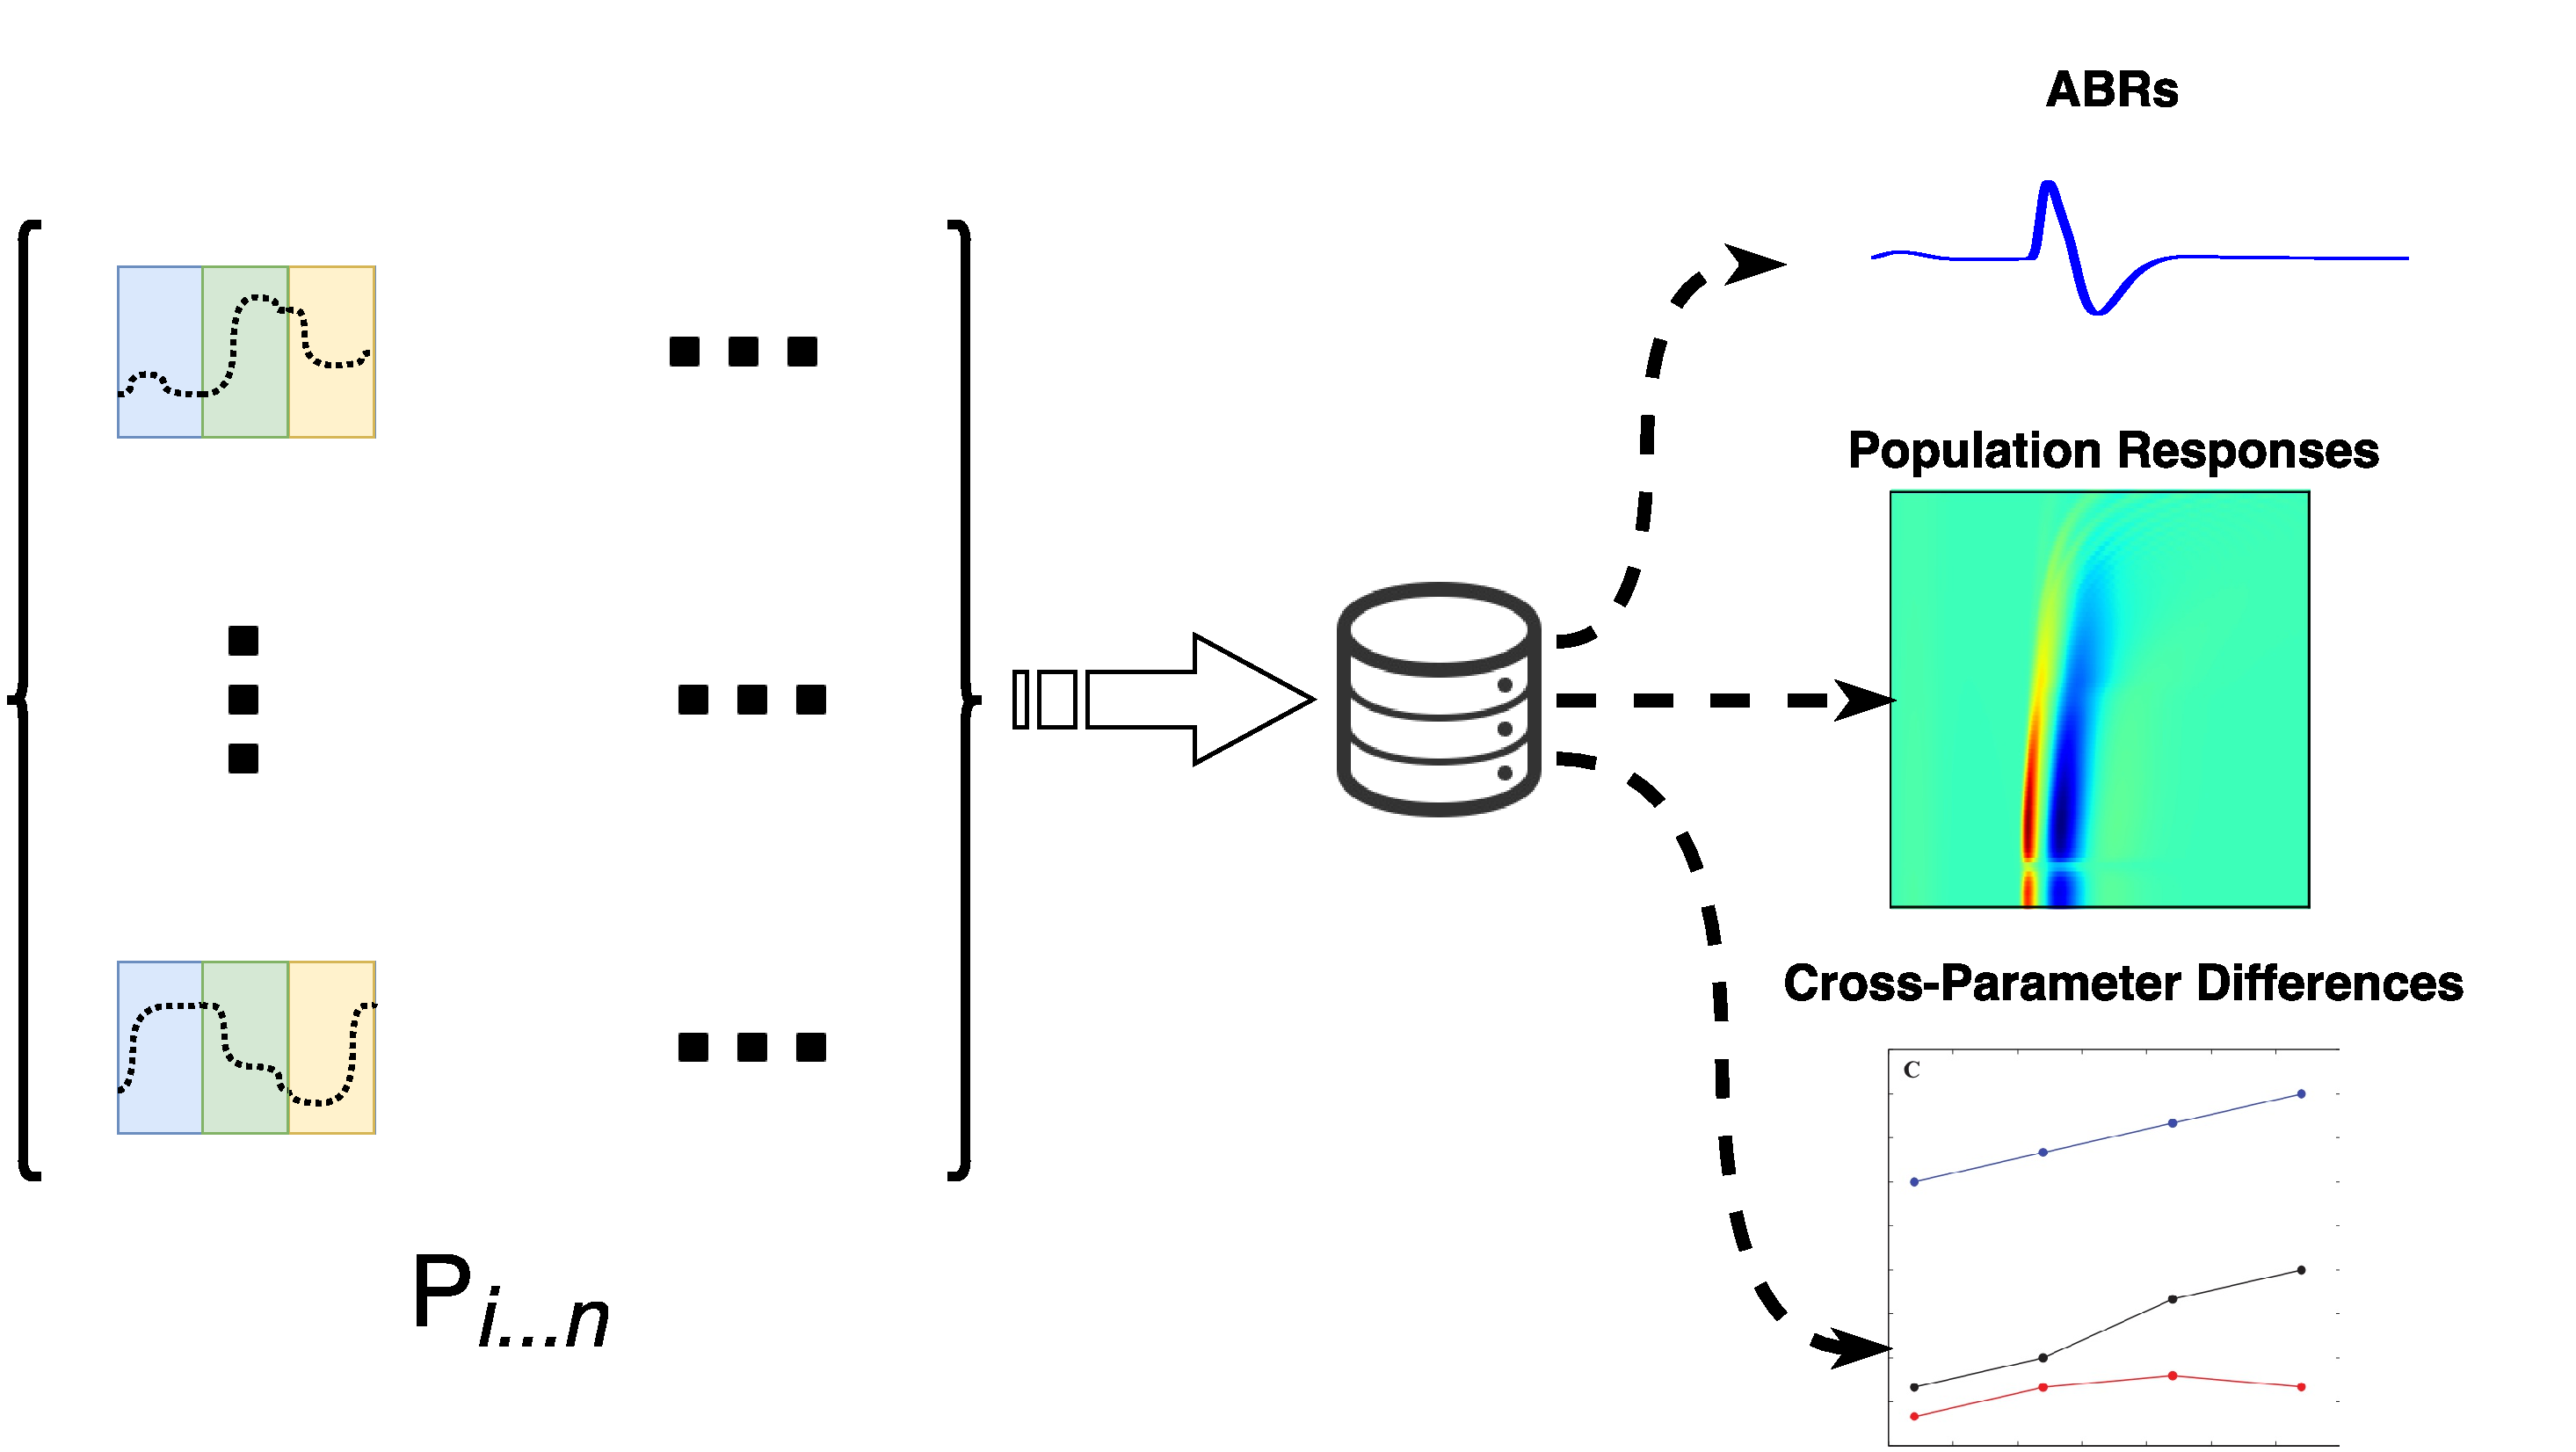
\includegraphics[width=0.95\textwidth]{pypet-workflow.pdf}
	\caption[Automated Exploration of Model Parameters]{\textbf{Automated exploration of model parameters} Each element P$_i$ in the matrix is a representation of one set of multiple parameter values that specify one trajectory through the parameter space.  A total of $N$ trajectories, where $N$ is the Cartesian product of the specified value ranges that a given parameter may take, are computed in parallel and stored in a database for further analysis.  Three possible analyses are shown: computation of a model ABR, visualization of population responses, and cross-parameter differences, or comparisons between trajectories. }
	\label{fig:pypet-overview}
\end{figure}
\subsection{Design of New Experiments} % (fold)
\label{sub:design_of_new_experiments}
While \autoref{chapter:Results} focuses on a particular combination of trajectories, designed to replicate and explore the contributions of different modeling considerations to a particular stimulus, the method presented in \autoref{sec:automated_parameter_exploration} is much more generally applicable.  Using Corti, one can easily design and run many other modeling experiments using these techniques for a wide variety of stimuli or parameter values without modification of the code of the core model functionality. 
